% The five joint types, and the two weld types that make them.
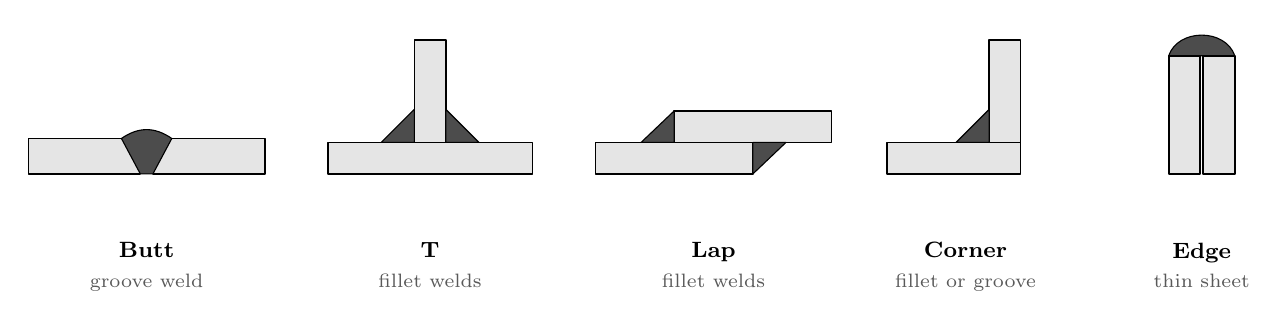
\begin{tikzpicture}[line join=round]
\tikzset{pl/.style={fill=black!10,draw=black,line width=0.6pt}, wd/.style={fill=black!70,draw=black,line width=0.4pt},
  ttl/.style={font=\footnotesize\bfseries,anchor=north}, sub/.style={font=\scriptsize,anchor=north,text=black!65,align=center}}
% butt
\begin{scope}
 \path[pl] (-1.5,0) rectangle (-0.08,0.45); \path[pl] (0.08,0) rectangle (1.5,0.45);
 \path[wd] (-0.08,0) -- (-0.32,0.45) .. controls (-0.1,0.6) and (0.1,0.6) .. (0.32,0.45) -- (0.08,0) -- cycle;
 \node[ttl] at (0,-0.75) {Butt}; \node[sub] at (0,-1.15) {groove weld};
\end{scope}
% T
\begin{scope}[xshift=3.6cm]
 \path[pl] (-1.3,0) rectangle (1.3,0.4); \path[pl] (-0.2,0.4) rectangle (0.2,1.7);
 \path[wd] (-0.2,0.4) -- (-0.62,0.4) -- (-0.2,0.82) -- cycle; \path[wd] (0.2,0.4) -- (0.62,0.4) -- (0.2,0.82) -- cycle;
 \node[ttl] at (0,-0.75) {T}; \node[sub] at (0,-1.15) {fillet welds};
\end{scope}
% lap
\begin{scope}[xshift=7.2cm]
 \path[pl] (-1.5,0) rectangle (0.5,0.4); \path[pl] (-0.5,0.4) rectangle (1.5,0.8);
 \path[wd] (-0.5,0.4) -- (-0.92,0.4) -- (-0.5,0.8) -- cycle; \path[wd] (0.5,0.4) -- (0.92,0.4) -- (0.5,0) -- cycle;
 \node[ttl] at (0,-0.75) {Lap}; \node[sub] at (0,-1.15) {fillet welds};
\end{scope}
% corner
\begin{scope}[xshift=10.6cm]
 \path[pl] (-1.2,0) rectangle (0.5,0.4); \path[pl] (0.1,0.4) rectangle (0.5,1.7);
 \path[wd] (0.1,0.4) -- (-0.32,0.4) -- (0.1,0.82) -- cycle;
 \node[ttl] at (-0.2,-0.75) {Corner}; \node[sub] at (-0.2,-1.15) {fillet or groove};
\end{scope}
% edge
\begin{scope}[xshift=13.4cm]
 \path[pl] (-0.42,0) rectangle (-0.02,1.5); \path[pl] (0.02,0) rectangle (0.42,1.5);
 \path[wd] (-0.42,1.5) .. controls (-0.3,1.85) and (0.3,1.85) .. (0.42,1.5) -- cycle;
 \node[ttl] at (0,-0.75) {Edge}; \node[sub] at (0,-1.15) {thin sheet};
\end{scope}
\end{tikzpicture}
